\documentclass[10pt,a4paper]{article}
\usepackage[utf8]{inputenc}
\usepackage{amsmath}
\usepackage{amsfonts}
\usepackage{amssymb}
\usepackage{makeidx}
\usepackage{graphicx}
\usepackage{lmodern}
\usepackage{listings}
\author{Andrea Colarieti Tosti}
\title{Rechenarchitekturen Tutorium 6 Lösung}

\begin{document}
\maketitle \newpage

\section{Aufgabe 29}
\subsection{a}
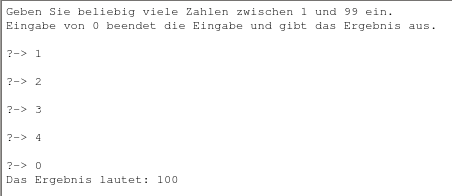
\includegraphics[scale=0.9]{Ergebnis.png} 

\subsection{b}
\begin{lstlisting}
# declaration der noetigen Strings die spaeter fuer die Kommunikation mit dem 
# user benutzt werden.
	.data

# reservieren eines speicherplatz fuer str1 
# asciiz terminiert das string mit dem Null_Byte 
# also erfolgt bei dem aufruf ascii gefolgt von asciiz eine implizite concatenation 
# der 2 strings in str1. 
# \n ist eine einrueckung
str1:	.ascii "Geben Sie beliebig viele Zahlen zwischen 1 und 99 ein.\n"	
	.asciiz "Eingabe von 0 beendet die Eingabe und gibt das Ergebnis aus.\n"

#platz reservieren fuer askstr 
askstr:	.asciiz "\n?-> "

#platz reservieren fuer errstring 
errstr:	.asciiz "Sie duerfen nur Zahlen zwischen 1 und 99 eingeben.\n"

#platz reservieren fuer answstr  
answstr:.asciiz "Das Ergebnis lautet: "

#platz reservieren fuer str2 
str2:	.asciiz "\n\n"


#implementation des programmes
	.text
	
#anfang main
#aufruf von main hier faengt das programm an zu arbeiten
main:

# laden 0 into $s0  
	li	$s0, 0
	
# laden 0 into $s1
	li	$s1, 0

# laden 4 into $v0 
	li	$v0, 4	
	
# laden des speichers an adresse str1 in $a0	
	la	$a0, str1       

# aufruf der betriebsystem funkionen	
# liest den wert im register $v0 und fuehrt die entsprechenden funktion aus 
# fuer diesen fall funkton nummer 4 print_sting liest string aus $a0
	syscall

#anfang loop 	
# loop wiederholt die ausf+hrung seines inhaltes bis eine bedingung eintrifft
loop:	

# laden der funktion print_string $v0 <- 4
	li	$v0, 4		

# laden des speicher an stelle askstr in $a0 fuer spaeteren syscall
	la	$a0, askstr     

# syscall print_string 
	syscall

# $v0 wird mit 5 befuellt Read-int : schreibt die User eingabe in $v0
	li	$v0, 5		

# read int ausfuehren	
	syscall

# lader der nummer 99 ins temporaeren speicher $t0
	li	$t2, 99
	
# sprung funktion sollte $v0 > $t2 sein geht es bei "error:	" weiter
# also wird hier die eingabe auf die einschraenkung geprueft 
# gelesene Zahl < t2 = 99
	bgt	$v0, $t2, error

# laden der nummer null ins temp speicherplatz $t2
	li	$t2, 0

# noch eine sicherheits pruefung ob die eingegebene zahl positiv ist 
# eingegebene Zahl < 0 => error
	blt	$v0, $t2, error

# sprung zu exit falls $v0 = null	
	beqz	$v0, exit

# addition speicherplatz $s1 wird mit $s1+1 befuellt
	addi	$s1, $s1, 1

# multiplikation $t2 wird ueberschrieben mit $v0*$v0 = $v0 quadrat
	mul	$t2, $v0, $v0
	
# multiplikation $t2 wird ueberschrieben mit $t2 * $s1
	mul	$t2, $t2, $s1

# addition $s0 <- $s0+$t2
	add	$s0, $s0, $t2

# jump back into loop : neustart
	j	loop

# anfang error
error:	
	
# laden der funktion print_string $v0 <- 4
	li	$v0, 4

# speicher bei der adresse errstr wird in $a0 geladen
	la	$a0, errstr	

# syscall 4 print_string
	syscall
	
# jump back into loop after erroneous imput
	j	loop

#anfang exit 
exit:	

# laden der funktion print_string $v0 <- 4 
	li	$v0, 4		

# $a0 wird mit answstr befuellt
	la	$a0, answstr    

# print_string answstr
	syscall

# laden des wert 1 in $v0 => print_int
	li	$v0, 1

# das wert $s0 wird mit dem wert aus $a0 befuellt .. $a0 = $s0
	move	$a0, $s0

# print result int
	syscall

# laden der funktion print_string $v0 <- 4 
	li	$v0, 4		

# $a0 wird mit str2 befuellt
	la	$a0, str2       
	
# print str2
	syscall
	
#laden 10 into $v0 => exit
	li	$v0, 10
# exit funktion ausfuehren	
	syscall

\end{lstlisting}

\subsection{c}
Die beschriebene funktion schaut wie folgt aus:\\
Seien die user eingaben definiert durch E = $\{e_1, e_2, ... e_n\}$, dann ist n die anzahl der eingaben.\\
Ergebnis = $ \sum_{i = 1}^n e_i^2 * i $

\newpage
\section{Aufgabe 30}
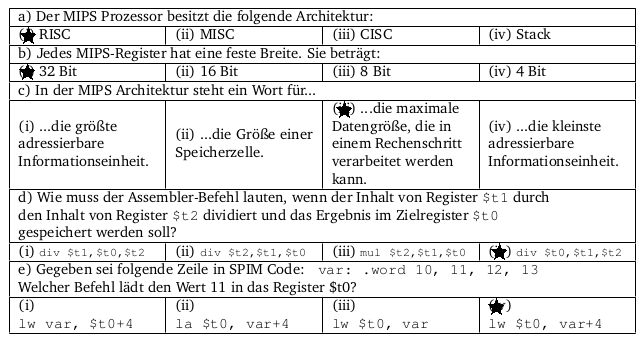
\includegraphics[scale=0.5]{A30.png} 


\end{document}